\documentclass[a4j,titlepage]{jsarticle}

\usepackage[dvipdfmx]{graphicx,xcolor}
\usepackage[top=20truemm,left=25truemm,right=25truemm]{geometry}
\usepackage{amsmath}
\usepackage{here}
\usepackage{comment}
\usepackage{url}
\usepackage{plistings}
\usepackage{tikz}
\usepackage[framemethod=tikz]{mdframed}

\renewcommand{\lstlistingname}{リスト}

\newcommand{\chuo}[1]{\multicolumn{1}{|c|}{#1}}
\newcommand{\inpt}[1]{\underline{#1}\,\setlength{\fboxsep}{1pt}\fbox{\small ↓}}

\lstdefinestyle{C}{
  language=C,
  basicstyle=\small\ttfamily,
  keywordstyle=\color[HTML]{0000E0},
  stringstyle=\color[HTML]{A31515},
  commentstyle=\upshape\color[HTML]{008000},
  frame=trbl,
  framesep=5pt,
  columns=[l]{fullflexible},
  numbers=left,
  xleftmargin=3zw,
  lineskip=-0.2ex,
  breaklines=true,
  showstringspaces=false,
  tabsize=4,
  keepspaces=true
}

\lstdefinestyle{text}{
  language=,
  basicstyle=\ttfamily,
  frame=trbl,
  framesep=5pt,
  columns=[l]{fullflexible},
  xleftmargin=3zw,
  lineskip=-0.2ex,
  showstringspaces=false,
  tabsize=4,
  keepspaces=true
}

\mdfsetup{
  skipabove=5pt,
  innertopmargin=10pt,
  innerbottommargin=10pt,
  roundcorner=10pt,
  font=\ttfamily
}


\begin{document}


\begin{titlepage}
  \title{\huge{シミュレーション} \\ \LARGE{---定積分と常微分方程式---}}
	\author{学籍番号:16426 \\ 4年 電子情報工学科 23番 \\ 福澤 大地}
	\date{提出日 : 2019年12月12日}
  \maketitle
\end{titlepage}


\section{目的}
コンピュータを用いて、数学的な問題の近似解を求める手法を学習する。

今回は、定積分と常微分方程式について数値積分を行う。
いくつかの手法を実装し、それぞれを比較することで、各手法の特徴や精度を確認する。


\section{開発環境}
プログラムの開発、実行を行った環境を表\ref{tb:kan}に示す。

\begin{table}[H]
  \centering
  \caption{開発環境}
  \label{tb:kan}

  \begin{tabular}{|l|l|}
    \hline
    CPU & Intel Core i5--7400 @ 3.0GHz \\ \hline
    メモリ & 8GB \\ \hline
    OS & Microsoft Windows 10 Home \\ \hline
    システム & 64bit \\ \hline
    コンパイラ & GCC 7.4.0 \\ \hline
  \end{tabular}
\end{table}


\section{課題1 : 台形公式}
\subsection{課題内容}
式\ref{eq:kadai1}について、台形公式を用いて数値積分を行う。

\begin{equation}
  \int_0^\frac{\pi}{6} \frac{dx}{\cos x}
  \label{eq:kadai1}
\end{equation}

\subsection{プログラムリスト}
課題1のプログラムリストをリスト\ref{lst:kadai1}に示す。

分割数を$n$, 分割幅を$h$とすると、台形公式は式\ref{eq:daikei}のように表せる。
この計算を\texttt{trapezoid}関数内で行うことで、定積分の近似解を導出している。

\begin{equation}
  \int_a^b f(x) dx \simeq \frac{h}{2} \left[ f(a) + 2 \sum_{j=1}^{n-1} f(jh) + f(b) \right]
  \label{eq:daikei}
\end{equation}

\lstinputlisting[style=C,caption=課題1のプログラム,label=lst:kadai1]{code/kadai01-2.c}

\subsection{実行結果}
課題1の実行結果をリスト\ref{lst:kekka1}に示す。

\begin{lstlisting}[style=text,caption=課題1の実行結果,label=lst:kekka1]
n =  1, S = 3.0000000000000000, e = -0.1415926535897931
n =  2, S = 3.1000000000000001, e = -0.0415926535897930
n =  4, S = 3.1311764705882354, e = -0.0104161830015577
n =  8, S = 3.1389884944910889, e = -0.0026041590987043
n = 16, S = 3.1409416120413889, e = -0.0006510415484042
n = 32, S = 3.1414298931749753, e = -0.0001627604148178
\end{lstlisting}

\subsection{考察}
式\ref{eq:kadai1}の解析解は、式\ref{eq:kaiseki1}のようになる。

\begin{align}
  \int_0^\frac{\pi}{6} \frac{dx}{\cos x} &= \left[ \frac{1}{2} \log \left( \frac{1 + \sin x}{1 - \sin x} \right) \right]_0^\frac{\pi}{6} \nonumber \\
  &= \frac{1}{2} \log 3
  \label{eq:kaiseki1}
\end{align}

リスト\ref{lst:kekka1}を見ると、$n$が大きくなるにつれ、数値解と解析解の差が少なくなっていることが分かる。
具体的には、分割数が2倍になると、誤差は約$1/4$になっていることが分かる。


\section{課題2 : シンプソンの公式}
\subsection{課題内容}
式\ref{eq:kadai2}について、シンプソン公式を用いて数値積分を行う。

\begin{equation}
  \int_0^\frac{\pi}{2} \sin x dx
  \label{eq:kadai2}
\end{equation}

\subsection{プログラムリスト}
課題2のプログラムリストをリスト\ref{lst:kadai2}に示す。

分割数を$n$, 分割幅を$h$とすると、シンプソン公式は式\ref{eq:simp}のように表せる。
この計算を\texttt{simpson}関数内で行うことで、定積分の近似解を導出している。

\begin{equation}
  \int_a^b f(x) dx \simeq \frac{h}{3} \left[ f(a) + 4 \sum_{j=1}^\frac{n}{2} f(2jh - 1)
  + 2 \sum_{j=1}^{\frac{n}{2}-1} f(2jh) + f(b) \right]
  \label{eq:simp}
\end{equation}

\lstinputlisting[style=C,caption=課題2のプログラム,label=lst:kadai2]{code/kadai02-2-double.c}

\subsection{実行結果}
double型の場合の実行結果をリスト\ref{lst:kekka2-d}, float型の場合の実行結果をリスト\ref{lst:kekka2-f}に示す。

\begin{lstlisting}[style=text,caption=課題2の実行結果(double型の場合),label=lst:kekka2-d]
n =  2, S = 1.0022798774922104, e = 0.0022798774922104
n =  4, S = 1.0001345849741938, e = 0.0001345849741938
n =  8, S = 1.0000082955239677, e = 0.0000082955239677
n = 16, S = 1.0000005166847066, e = 0.0000005166847066
n = 32, S = 1.0000000322650009, e = 0.0000000322650009
\end{lstlisting}

\begin{lstlisting}[style=text,caption=課題2の実行結果(float型の場合),label=lst:kekka2-f]
n =  2, S = 1.0022798776626587, e = 0.0022798776626587
n =  4, S = 1.0001345872879028, e = 0.0001345872879028
n =  8, S = 1.0000083446502686, e = 0.0000083446502686
n = 16, S = 1.0000005960464478, e = 0.0000005960464478
n = 32, S = 1.0000001192092896, e = 0.0000001192092896
\end{lstlisting}

\subsection{考察}
式\ref{eq:kadai2}の解析解は、式\ref{eq:kaiseki2}のようになる。

\begin{align}
  \int_0^\frac{\pi}{2} \sin x dx &= \left[ -\cos(x) \right]_0^\frac{\pi}{2} \nonumber \\
  &= 1
  \label{eq:kaiseki2}
\end{align}

リスト\ref{lst:kekka2-d}を見ると、$n$が大きくなるにつれ、数値解と解析解の差が少なくなっていることが分かる。
具体的には、分割数が2倍になると、誤差は約$1/16$になっていることが分かる。

また、リスト\ref{lst:kekka2-d}とリスト\ref{lst:kekka2-f}比べると、float型で計算を行ったときの方が誤差が大きくなっていることが分かる。
特に、$n=32$の場合を比較すると、float型の誤差はdouble型に比べて約4倍と、非常に大きな差が生じている。


\section{課題3--5 : 常微分方程式}
\subsection{課題内容}
式\ref{eq:kadai3}をオイラー法、ホイン法、ルンゲ・クッタ法を用いて解く。
ただし、$t = 0$のとき$u = 1$とする。

\begin{equation}
  \frac{du}{dt} = u
  \label{eq:kadai3}
\end{equation}


\subsection{プログラムリスト}
課題3のプログラムリストをリスト\ref{lst:kadai3}に示す。

オイラー法は式\ref{eq:euler}, ホイン法は式\ref{eq:heun}, ルンゲ・クッタ法は式\ref{eq:runge}のように表せる。
これらの計算を、それぞれ\texttt{euler}, \texttt{heun}, \texttt{runge\_kutta}関数内で行うことで、解を導出している。

\begin{equation}
  \begin{aligned}
    x_{i+1} &= x_i + h \\
    y_{i+1} &= y_i + h f(x_i, \, y_i)
  \end{aligned}
  \label{eq:euler}
\end{equation}

\begin{equation}
  \begin{aligned}
    x_{i+1} &= x_i + h \\
    k_1 &= h f(x_i, \, y_i) \\
    k_2 &= h f(x_i + h, \, y_i + k_1) \\
    y_{i+1} &= y_i + \frac{1}{2} (k_1 + k_2)
  \end{aligned}
  \label{eq:heun}
\end{equation}

\begin{equation}
  \begin{aligned}
    x_{i+1} &= x_i + h \\
    k_1 &= h f(x_i, \, y_i) \\
    k_2 &= h f(x_i + \frac{h}{2}, \, y_i + \frac{k_1}{2}) \\
    k_3 &= h f(x_i + \frac{h}{2}, \, y_i + \frac{k_2}{2}) \\
    k_4 &= h f(x_i + h, \, y_i + k_3) \\
    y_{i+1} &= y_i + \frac{1}{6} (k_1 + 2 k_2 + 2 k_3 + k_4)
  \end{aligned}
  \label{eq:runge}
\end{equation}

\lstinputlisting[style=C,caption=課題3--5のプログラム,label=lst:kadai3]{code/kadai03-3.c}

\subsection{実行結果}
\begin{lstlisting}[style=text,caption=課題3--5の実行結果,label=lst:kekka3]
オイラー法
i =  0, t = 0.0000000000000000, u = 1.0000000000000000, e = 0.0000000000000000
i =  1, t = 0.1000000000000000, u = 1.1000000000000001, e = -0.0051709180756476
i =  2, t = 0.2000000000000000, u = 1.2100000000000002, e = -0.0114027581601697
i =  3, t = 0.3000000000000000, u = 1.3310000000000002, e = -0.0188588075760030
i =  4, t = 0.4000000000000000, u = 1.4641000000000002, e = -0.0277246976412702
i =  5, t = 0.5000000000000000, u = 1.6105100000000001, e = -0.0382112707001281
i =  6, t = 0.6000000000000000, u = 1.7715610000000002, e = -0.0505578003905087
i =  7, t = 0.7000000000000000, u = 1.9487171000000001, e = -0.0650356074704765
i =  8, t = 0.7999999999999999, u = 2.1435888100000002, e = -0.0819521184924672
i =  9, t = 0.8999999999999999, u = 2.3579476910000001, e = -0.1016554201569493
i = 10, t = 0.9999999999999999, u = 2.5937424601000001, e = -0.1245393683590450

ホイン法
i =  0, t = 0.0000000000000000, u = 1.0000000000000000, e = 0.0000000000000000
i =  1, t = 0.1000000000000000, u = 1.1050000000000000, e = -0.0001709180756477
i =  2, t = 0.2000000000000000, u = 1.2210250000000000, e = -0.0003777581601698
i =  3, t = 0.3000000000000000, u = 1.3492326250000000, e = -0.0006261825760032
i =  4, t = 0.4000000000000000, u = 1.4909020506249999, e = -0.0009226470162704
i =  5, t = 0.5000000000000000, u = 1.6474467659406249, e = -0.0012745047595033
i =  6, t = 0.6000000000000000, u = 1.8204286763643904, e = -0.0016901240261185
i =  7, t = 0.7000000000000000, u = 2.0115736873826515, e = -0.0021790200878251
i =  8, t = 0.7999999999999999, u = 2.2227889245578298, e = -0.0027520039346376
i =  9, t = 0.8999999999999999, u = 2.4561817616364019, e = -0.0034213495205475
i = 10, t = 0.9999999999999999, u = 2.7140808466082240, e = -0.0042009818508211

ルンゲ・クッタ法
i =  0, t = 0.0000000000000000, u = 1.0000000000000000, e = 0.0000000000000000
i =  1, t = 0.1000000000000000, u = 1.1051708333333334, e = -0.0000000847423143
i =  2, t = 0.2000000000000000, u = 1.2214025708506946, e = -0.0000001873094753
i =  3, t = 0.3000000000000000, u = 1.3498584970625378, e = -0.0000003105134654
i =  4, t = 0.4000000000000000, u = 1.4918242400806858, e = -0.0000004575605845
i =  5, t = 0.5000000000000000, u = 1.6487206385968383, e = -0.0000006321032899
i =  6, t = 0.6000000000000000, u = 1.8221179620919332, e = -0.0000008382985757
i =  7, t = 0.7000000000000000, u = 2.0137516265967768, e = -0.0000010808736999
i =  8, t = 0.7999999999999999, u = 2.2255395632923154, e = -0.0000013652001520
i =  9, t = 0.8999999999999999, u = 2.4596014137800708, e = -0.0000016973768786
i = 10, t = 0.9999999999999999, u = 2.7182797441351658, e = -0.0000020843238793
\end{lstlisting}

\subsection{考察}
リスト\ref{lst:kadai3}の3つの手法の実行結果を見比べると、オイラー法よりホイン法、ホイン法よりルンゲ・クッタ法の方が誤差が少ないことが分かる。
これは$i$が大きくなるにつれて顕著に現れる。

オイラー法は$i$に1つ増えるにつれて一定して誤差が増えている。つまり、

$h = 0.1$, $h = 0.05$とし、オイラー法で計算した数値解と、解析解を比較したグラフを図\ref{fig:kadai3}に示す。


\begin{figure}[H]
  \centering
  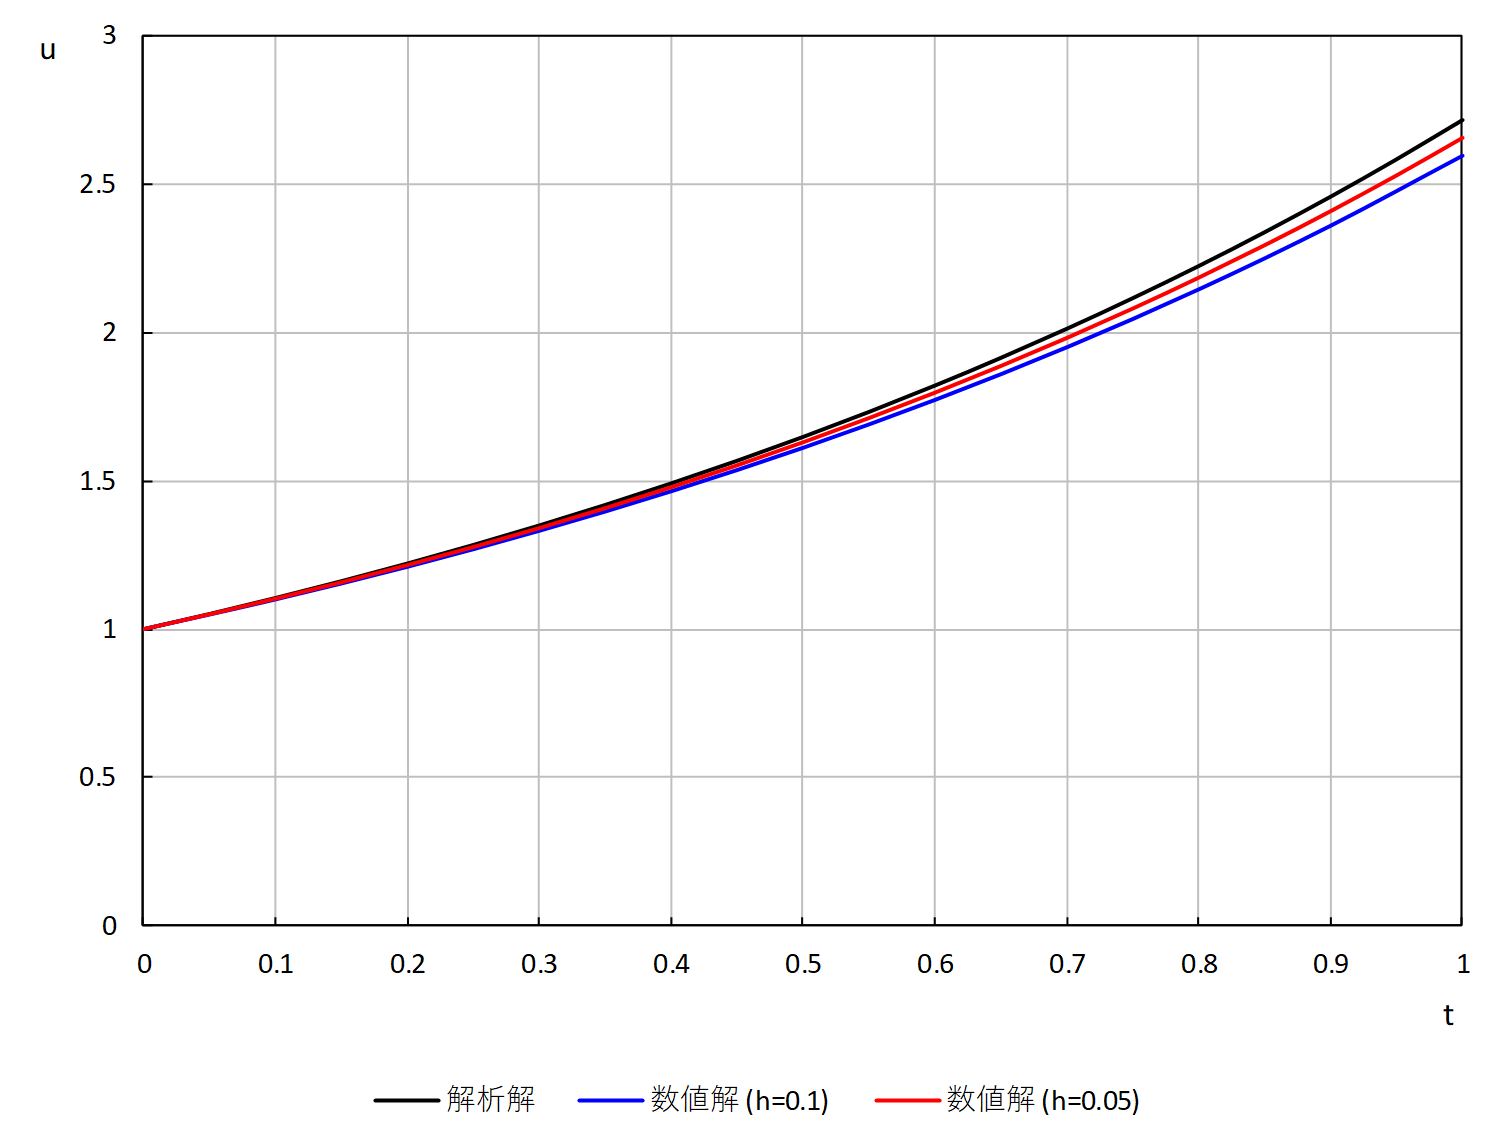
\includegraphics[width=15cm]{kadai3.png}
  \caption{オイラー法の数値解と解析解}
  \label{fig:kadai3}
\end{figure}


\end{document}
